In this chapter the implementation of the backend of the system, and the decisions made during this, is presented and described. The first section explains and argues about the choice of server hosting. This is then followed by descriptions about the different services that has been utilized to implement the backend. After this the implementation and layout of the API is presented, with the different functionality surrounding it, such as \textit{authentication} and the database. Finally the implementation of the personal assistant and IoT is described. 

\section{Choice of Server Hosting}\label{sec:server-choice}
Two different options were investigated with regards to hosting the web service. The first option researched was to host the system on a server. This could either be done as a dedicated or virtual server. The second option was to host it on a cloud computing platform.

Hosting the web service on a server would allow for the control panel, API and database to be hosted in one place. However, this solution would not be very scalable out of the box, as the system would be limited by a physical or virtual server. More virtual machines could be started, but would require using development time to setup the virtual server to automatically handle load balancing.

The alternative option was to use a cloud hosting solution. Cloud hosting solutions offer compute services, which is code that can be run in the cloud while being serverless. Serverless means that the whole management aspect of allocating resources to run the code is handled by the cloud provider. This would allow the code to scale, as it would not be dependent on the underlying server, or other running code, and a theoretically infinite number of instances could be run in parallel. Other resources such as databases would be hosted independently, and could then be accessed by using various endpoints.

In this project, it was chosen to use a serverless cloud hosting solution, because of the high flexibility and scalability. Furthermore, it allows for less time spent setting up a server and the different solutions needed for a project of this type.

A large variety of cloud hosting solutions exist. Two of the major ones are Amazon Web Services (AWS) and Google Cloud. Of these two, it was decided to develop the web service using AWS, since this gave us access to all the services needed to implement both the web service, through an API and a smart assistant, using Amazon Alexa. This choice made it possible to host all of the services, for both the API and smart assistant, in one place. The implementation of the Alexa smart assistant, is described in chapter \ref{sec:alexa}.

\section{Amazon Web Services}\label{sec:aws}
Amazon Web Services (AWS) contains several different services and solutions, some of which was used to implement the backend of the project. These are described in this section.

\subsection{Lambda}
Lambda functions are pieces of code that can be called from another AWS service, or directly over the internet. They can be programmed using Java, C\#, Python, and Node.js. Since there is no real server for the script to run on, there is no system to handle dependencies, because of this, these have to be uploaded together with the script for each Lambda. The code that should be run on a lambda function could also be uploaded to S3, and have Lambda fetch it every time it needs to run the code. The purpose of S3 is further explained in section \ref{s3}.

It is possible to control the Lambdas, limit how much RAM a Lambda can use to a maximum of 1.5GB of memory, and how long they can run before they should timeout to a limit of 5 minutes. Security policies can also restrict the lambdas such that they can only interact with other specific AWS services inside a VPC as explained in \ref{ec2}. 

\subsection{ARN}
ARN is short for Amazon Resource Name. It is a way to identify a resource on AWS, such as the Lambda functions used in this project. The ARN is unique across all AWS services and users. The structure of an ARN varies depending on the service but usually follows the structure

\texttt{arn:partition:service:region:account-id:resource}

All ARNs start with \texttt{arn}, followed by a \texttt{partition}, which for most cases is \texttt{aws}. The \texttt{service} is the AWS service it belongs to, such as \texttt{s3}, \texttt{iam}, \texttt{rds} or any other AWS service. \texttt{region} is the region where the resource is located. For some AWS services, the resource is only made available in specified regions. The \texttt{account-id} is the id of the AWS user the resource belongs to. The \texttt{resource} can have different forms depending on what service it belongs to. Not all services makes use of all parts since, as a service such as \texttt{IAM} is region independent.

\subsection{EC2}\label{ec2}
EC2 stands for Amazon Elastic Cloud Compute, and is a Virtual Computing Environment that can host virtual machines in a scalable fashion. It is also used for managing security groups that allow access to specific VPCs. VPC is short for Virtual Private Cloud, and is an isolated environment where certain AWS services can run disconnected from the surrounding world. As a result, AWS services inside and outside the VPC cannot interact with each other.
The VPC is necessary because certain services such as databases should not be directly visible to the outside world. Some AWS services such as lambda functions are configured to either run inside or outside the VPC. A lambda running outside the VPC can start another lambda function that can run inside the VPC to access internal resources, and have it return the result out of the VPC on termination.

\subsection{RDS}
RDS is shorthand for Relational Database Service, and can be used to create instances of databases. It is possible to host most common relational database types, including PostgreSQL, which has been chosen to use in this project. It is also possible to specify how much processing power the database has, as well as how much storage it should have access to. This allows for the flexible scaling needed in this project.

RDS uses EC2 security groups to control what can access databases as mentioned in \ref{ec2}. This means that every connection to the RDS has a specific rule - otherwise no connection is allowed. %If for example access to the RDS was required from a personal computer, the specific IP address would have to be white listed. AWS Lambda Functions also need to be part of a security group and run on an VPC to access the database.

\subsection{API Gateway}
API Gateway was used to create a REST API. Using API Gateway, it is possible to specify which resources the API should have, as well as what methods each resource has access to. The API Gateway can interact with many of the AWS systems through the API. The API Gateway also allows restriction of the API using authentication, such that API keys are required, and only specific users can use specific methods. API Gateway also gives full control over incoming and outgoing data, and how it is formatted.

\subsection{IAM}\label{sec:iam}
Amazons IAM (Identity and Access Management) service is a tool for administrating permissions for a system. In AWS it is more specifically used for two purposes: to manage the different services available to a developer through AWS, and to control access in the authorization layer of the API Gateway. Both of these cases are used in this project. The first is used to manage the different developer accounts used by the group throughout development. The second is used during authorization of an API call, to define which methods the user sending the request has access to. This is done through an authorizer, as described in section \ref{sec:authentication}, by it returning an IAM resource \cite{aws:iamres}.


\subsection{SNS}\label{sns_service}
SNS stands for Simple Notification Service, and is a tool that provides functionality for sending messages such as SMS, Email and App notifications. SMS and email is sent out directly from SNS, but it is unable to send notifications directly to the users smartphones. It needs to send the notifications over Google Cloud Messaging, Firebase Cloud Messaging, described in section \ref{sec:fcm}, or Apple Developer to reach Android and iOS devices.
SNS can create an application for each use case, such as Firebase and Apple Developer, to specify how it should send messages to devices in that application. Smartphones are added to an application by using their device identification token, and are then assigned an ARN within the application, such that the system can refer directly to that specific device.

\subsection{S3} \label{s3}
S3 stands for Simple Storage Service and is meant for storing and retrieving data. Use cases include: storing files for sharing, scripts for use with AWS Lambda Functions and HTML, CSS and JavaScript files for static websites. S3 is the recommended way to host a website using AWS, such as the one needed for the control panel \cite{aws:webhosting}. S3 makes use of buckets to store collections of files. Each bucket has a name that is unique across all of S3. Within each bucket it is possible to control the availability of different files, and limit who can upload and edit files, and when files can expire.\\
Websites hosted with S3 are also scalable, as it can make the files available on more servers as demand increases.

S3 is not the only way to host files on AWS as it offers different solutions. EFS is another storage solution used for EC2 storage, while Glacier is used for long term storage and achieving.

\subsection{Communication Between Services}\label{sec:communication-services}
All of the AWS services work together to form the fall detection service.

\begin{figure}[H]
    \centering
    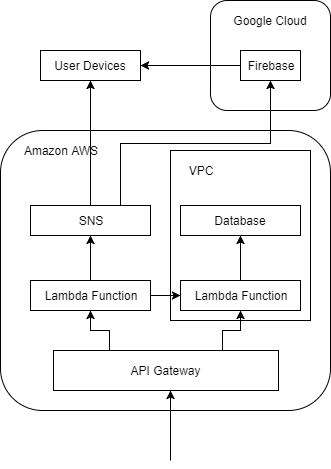
\includegraphics[scale=0.7]{Figures/aws_diagram.png}
    \caption{Flow of AWS Services}
    \label{fig:aws_diagram}
\end{figure}

Figure \ref{fig:aws_diagram} shows the order in which the different services are called. All requests from the control panel and devices goes through the API Gateway. The API Gateway then forwards the request data to the connected lambda function. The Lambda Functions inside the VPC can access the database, perform writing or reading, and return the related objects.\\
The AWS Lambda Function outside the VPC can call lambda functions within the VPC, or AWS SNS where it can send notifications (Smart phone notification) and SMS messages. For notifications to Android devices it needs to call Firebase from Google Cloud. The messages are then sent out to the users devices as needed.

\section{API}
In this section the API and underlying implementation is described. First an overview of how input is handled and the general structure of the lambda functions used for the API calls, is described, after which the different endpoints and their implementation is presented.

\subsection{Input mapping} \label{api:mapping}
Mapping is used to map headers, body and URL parameters into a dictionary that the API can forward to the AWS Lambda Function. The mapping ensures that the input parameters are available by their expected name in the lambda function. Should the names of the underlying implementation change, the mapping can be updated without the parameter names in the API needing to be changed.\\
The mapping also allows for some level of modification of the input before passing it on.

\subsection{Structure}
All lambda functions follow the same general structure to make input and output with the API simple and consistent.

\begin{figure}[H]
    \centering
    \begin{lstlisting}[language=Python]
        def lambda_handler(event, context)
            try:
                input_var1 = event["input_var1"]
                ...
                
                if not input_var1:
                    # Return error since we have unassigned variables
                    
                # LOGIC
                
                return respond(statuscode, serializedobject)
            except:
                return respond(statuscode, errorobject)
    \end{lstlisting}
    \caption{The base structure of a lambda function}
    \label{fig:samplelambdafunction}
\end{figure}

As seen on figure \ref{fig:samplelambdafunction} a \textit{lambda\_handler} method takes an event and a context. 
All input happens through the event, which is a (string, string) dictionary containing the mapped input. 
The context is never used in this project, but contains information about the lambda function itself, such as AWS request id, available memory, and remaining running time until it gets terminated for timeout.
The lambda function always returns an HTTP request response with a status code, body and headers.

Most \textit{lambda\_handler} methods follow the same general structure. First, all arguments are retrieved from the event parameter, and assigned to local parameters, and if an object from the model is expected, the value is deserialized. After this some error handling is done, depending on the input, before the main logic of the lambda is executed.

A \textit{Response} is built using a status code, and the data that it should return. In this project all lambda functions return an object as shown on figure \ref{table:api}.

When returning an error, an object is constructed that follow the same pattern as the otherwise correct object, but with a negative ID, and most other fields as empty strings or arrays, since the error does not contain any info.
The status code returned for a success is always 200, while a status code 400 is for failure. Any other status code returned from the server as a result of problems outside the reach of the server implementation.

\subsection{Endpoints}
The API consists of endpoints that allow access to the different resources available. Each endpoint is open to HTTP request methods, and has both input and output. All endpoints are accessed from a specific API Gateway URL.

\begin{table}[H]
    \centering
    \begin{tabular}{|l|p{2cm}|p{2cm}|p{2cm}|p{2cm}|} \hline
         Resource & GET & POST & PUT & DELETE \\ \hline
         /Citizen/\{id\} & In: \newline - Citizen\_id \newline Out:  \newline - Citizen & \cellcolor{gray!40} & \cellcolor{gray!40} & \cellcolor{gray!40} \\ \hline
         /Contact/\{id\} & In: \newline - Contact\_id \newline Out: \newline - Contact & \cellcolor{gray!40} & \cellcolor{gray!40} & \cellcolor{gray!40} \\ \hline
         /Contact/ & In: \newline - \newline Out:  \newline - [Contact] & \cellcolor{gray!40} & \cellcolor{gray!40} & \cellcolor{gray!40} \\ \hline
         /Citizen/\{id\}/Alarm & In: \newline - Citizen\_id \newline Out: \newline - Alarm & In: \newline - Citizen\_id \newline Out: \newline - Alarm & In: \newline - Alarm \newline Out: \newline - Alarm & In: \newline - Alarm \newline Out: \newline - Alarm \\ \hline
         /.../\{id\}/Device & \cellcolor{gray!40} & In: \newline - Device \newline - User\_id \newline Out: \newline - Device & In: \newline - Device \newline Out: \newline - Device & In: \newline - Device \newline Out: \newline - Device \\ \hline
         /User & In: \newline - email \newline - password \newline Out: \newline - User & In: \newline - User \newline Out: \newline - User & In: \newline - User \newline Out: \newline - User & In: \newline - User \newline Out: \newline - User \\ \hline
    \end{tabular}
    \caption{API calls}
    \label{table:api}
\end{table}

Table \ref{table:api} shows the different endpoints of the API and their input and output. When an endpoint returns an object from the model, it refers to the full serialized objects. Even when dealing with errors or representing deleted content, the models are used, just with empty fields where possible, and negative IDs. This is done to keep the responses consistent. In table \ref{table:api} if output is in a \[\], it means the output value is a list.

The following sub sections describe each of the endpoints, and their purposes. The non-trivial endpoints also contains some explanation of their implementation.

\subsubsection{/User}
The user resource is used for creating and editing users. For a user to login to the system, they must make a \textit{GET} request to the user endpoint, with their email and password.

\subsubsection{Password security}
When a user creates a user in the system, they are required to make a password. Since storing passwords in plaintext is a bad practice, a few steps has to be taken to keep the users information safe. To keep these passwords secure, it is salted and hashed, such that only the salted and hashed version of the password is saved in the database.

\begin{figure}[H]
    \centering
    \begin{lstlisting}[language=Python]
    def get_salt():
        return uuid.uuid4().hex


    def hash_password(password, salt):
        return hashlib.sha512((password + salt).encode('utf-8')).hexdigest()
    \end{lstlisting}
    \caption{Functions for getting salt and hashed password}
    \label{fig:passwordhashing}
\end{figure}

The salt for a password is generated by using Pythons built-in uuid library\cite{Python:UUID}. The library documentation recommends uuid4 for a random UUID. This function returns a string of 32 hexadecimal digits. The salts are used to ensure that even if two users has the same password, it is stored as different strings in the database. When the user has been created, the password is run though a hashing function, seen on \ref{fig:passwordhashing}, with the salt.

On a login request, the password the user used for the request is hashed with the same salt, and the two hashed passwords are compared. If the hashed passwords are identical the user is returned. Otherwise an empty user is returned, which indicates an error or invalid credentials on login.

While hashing libraries exist such as bcrypt \cite{bcrypt} that offers many advanced solutions for password hashing, a simpler solution was chosen. Bcrypt also stores the hash and salt together in the database, making it more difficult to port in the future, should another library need access to the login information in the database.

\subsubsection{/Citizen/\{id\}}
When a user of role \textit{useradmin} or \textit{citizenadmin} need to request an individual citizen, it is done by adding the citizens id as part of the request.

\subsubsection{/Contact/\{id\}}
As with the Citizen endpoint, a specific contact is requested by adding the contact's id as part of the request.

\subsubsection{/Contact}
When administrating a citizen through the control panel, it is necessary to get all contacts in the system. This endpoint returns all contacts in the system, through a \textit{Get} request.

\subsubsection{/Citizen/\{id\}/Alarm}
This endpoint is used when a citizen raises an alarm. No alarm object is expected as input, since the current citizen is specified directly in the URL. When the system creates an alarm the lambda function calls a second lambda function. This is required since it is needed to both update the database and send out potential messages through SNS, which, as described in section \ref{sec:communication-services}, is not possible through the same lambda function.

\begin{figure}[H]
    \centering
    \begin{lstlisting}[language=Python]
    lambda_client = boto3.client('lambda',
        region_name=region_name,
        aws_access_key_id=aws_access_key_id,
        aws_secret_access_key=aws_secret_access_key)

    arg = bytes(json.dumps({"id": ctz_id}), 'utf-8')
    response = lambda_client.invoke(
        FunctionName=arn_alarm_create_endpoint,
        InvocationType="RequestResponse",
        Payload=arg)

    data = response["Payload"].read().decode()
    \end{lstlisting}
    \caption{Code for starting a lambda function from within another lambda function}
    \label{fig:startlambda}
\end{figure}

This process of calling a second lambda function from within a lambda function, is shown on \ref{fig:startlambda}. The second lambda function can then create the alarm and store it in the database, before returning to the original lambda function.

When sending a message to a device, it is necessary to have a means to identify which device to send it to.

\begin{figure}[H]
    \centering
    \begin{lstlisting}[language=Python]
    def push_message(endpoint_arn, message):
        sns_client = boto3.client(
            'sns',
            region_name=region_name,
            aws_access_key_id=aws_access_key_id,
            aws_secret_access_key=aws_secret_access_key
        )
    
        return sns_client.publish(
            TargetArn=endpoint_arn,
            MessageStructure='string',
            Message=message
        )
    \end{lstlisting}
    \caption{Sending a notification to a device using SNS}
    \label{fig:sns_notification}
\end{figure}

As seen on figure \ref{fig:aws_diagram}, SNS sends the message via Firebase, as described in section \ref{sec:fcm}, which uses an ARN to identify which android device it should send the message to. Figure \ref{fig:sns_notification} shows that when sending a message, only the ARN for the token is needed, as explained in \ref{sns_service}. While the Application ARN is needed when adding the token, the tokens ARN can be used directly afterwards when sending a notification, or updating the token in case it has changed.

\begin{figure}[H]
    \centering
    \begin{lstlisting}[language=Python]
        for c in alm.activatedby.contacts:
            for d in c.devices:
                if d.devicetype == "appdevice":
                    if not d.arn or not d.token:
                        continue
                    try:
                        push_message(d.arn, alm.serialize())
                    except:
                        print("ARN NOT ACTIVE: " + d.arn)
                elif d.devicetype == "smsdevice":
                    send_sms(d.phone_number, c.activatedby.name + " has had an falling accident, and requests help.")

        for d in alm.activatedby.devices:
            if d.devicetype == "iftttdevice":
                urllib.request.urlopen(
                    "https://maker.ifttt.com/trigger/fall_detected/with/key/" + d.token).read()
    \end{lstlisting}
    \caption{Sending notifications out to all contacts, and triggering all IFTTT hooks}
    \label{fig:notify_contacts}
\end{figure}

Figure \ref{fig:notify_contacts} shows the code for sending notifications after a citizen has had a falling accident. The code makes sure that all contacts related to the citizen are notified through their devices. For smartphone notifications it must make sure that the ARN exist, and in the case that the ARN cannot be reached because it is not active, it should log it. When sending an SMS it is important that the provided number also has the correct country code, as SNS can send SMS to the entire world, and would not know where to send it otherwise.

\subsubsection{/.../\{id\}/Device}
This endpoint is used by both Citizen and Contact to create and update devices. While the device resource is the same for both citizens and contacts, it was added to both of them to make the API more transparent.

This endpoint is also used by the control panel when setting up an Alexa or IFTTT device, as described in section \ref{chap:controlPanel}. The smartphone app is automatically added as a device and removed from the system as users log in and out from the app. 

\subsection{Authentication}\label{sec:authentication}
To ensure that users only access the parts of the API that they are allowed to, an authentication layer has been added. When a user logs in, they are given an authentication token. This token needs to be provided together with any request made to the rest of the API to ensure that they only have access to the endpoints that they are allowed to. It also prevents unauthorized people from doing malicious things. Table \ref{table:auth} shows which resources and methods each user can access. A user is assigned a token when they log in to the system through the API.

\begin{table}[H]
\centering

\begin{tabular}{|l|l|l|l|l|l|}
\hline
                    & Citizen                                                     & Contact                                                     & User admin                                                  & Citizen admin            & No auth                                        \\ \hline
/citizen/id/        & GET                                                         & \cellcolor[HTML]{9B9B9B}{\color[HTML]{9B9B9B} }             & GET                                                         & GET                      & \cellcolor[HTML]{9B9B9B}                                 \\ \hline
/contact/id/        & \cellcolor[HTML]{9B9B9B}                                    & \cellcolor[HTML]{9B9B9B}{\color[HTML]{9B9B9B} }             & \cellcolor[HTML]{9B9B9B}                                    & \cellcolor[HTML]{9B9B9B} & \cellcolor[HTML]{9B9B9B}                                 \\ \hline
/contact/           & GET                                                         & GET                                                         & GET                                                         & GET                      & \cellcolor[HTML]{9B9B9B}                                 \\ \hline
/citizen/id/alarm/  & POST                                                        & \begin{tabular}[c]{@{}l@{}}GET\\ POST\end{tabular}          & \cellcolor[HTML]{9B9B9B}                                    & \cellcolor[HTML]{9B9B9B} & \cellcolor[HTML]{9B9B9B}                                 \\ \hline
/citizen/id/device/ & \begin{tabular}[c]{@{}l@{}}POST\\ PUT\\ DELETE\end{tabular} & \cellcolor[HTML]{9B9B9B}                                    & \begin{tabular}[c]{@{}l@{}}POST\\ PUT\\ DELETE\end{tabular} & \cellcolor[HTML]{9B9B9B} & \cellcolor[HTML]{9B9B9B}                                 \\ \hline
/contact/id/device/ & \cellcolor[HTML]{9B9B9B}                                    & \begin{tabular}[c]{@{}l@{}}POST\\ PUT\\ DELETE\end{tabular} & \begin{tabular}[c]{@{}l@{}}POST\\ PUT\\ DELETE\end{tabular} & \cellcolor[HTML]{9B9B9B} & \cellcolor[HTML]{9B9B9B}                                 \\ \hline
/user/              & \cellcolor[HTML]{9B9B9B}                                    & \cellcolor[HTML]{9B9B9B}                                    & \cellcolor[HTML]{9B9B9B}                                    & \cellcolor[HTML]{9B9B9B} & \begin{tabular}[c]{@{}l@{}}GET\\ POST\\ PUT\end{tabular} \\ \hline
\end{tabular}
\caption{Table of user authorizations}
\label{table:auth}
\end{table}

The AWS API Gateway includes a tool to add authorizers to an API. This is done by defining a lambda function to handle the authorization request (also called an authorizer), which returns an IAM resource, which is explained in section \ref{sec:iam}. The authorizer takes an authentication token as a parameter, the source of which must be defined when setting up the authorizer, in this case, the source is a header called \textit{token}.

The token is generated using the JSON Web Tokens (JWT) standard \cite{JWT}. Due to the compact size of a JWT, this makes it possible to send it through the request header. Furthermore, it is self contained, meaning that the token contains all the required information, which results in that a call to the database is not required during the authorization step. Each token is signed using a secret string.

\begin{figure}[H]
    \centering
    \begin{lstlisting}[language=Python]
    Header:
    {
        "typ": "JWT",
        "alg": "HS256"
    }
    
    Payload:
    {
        "user_id": "234",
        "user_role": "citizen"
    }
    
\end{lstlisting}
    \caption{Decoded JSON Web Tokens}
    \label{fig:jwt-decoded}
\end{figure}

A JWT consists of three parts, namely the header, payload and signature. An example of a JWT, used in the API test, can be found on figure \ref{fig:jwt-decoded}. The header contains information about the type of the token, which is \textit{JWT}, and the hashing algorithm used, in this case \textit{HS256}. The payload contains the data that the token contains. In this example it contains a user id and user role, used by the authorizer to create the IAM. The third part, which is not shown in the example, is the signature part. This part contains information needed to verify the token, including the secret string needed to verify the token.

The three parts of the JWT is encoded and separated by a period ('.'). The encoded version of the example on figure \ref{fig:jwt-decoded} can be found on figure \ref{fig:jwt-encoded}.

\begin{figure}[H]
    \centering
    \begin{lstlisting}[language=Python]
    eyJ0eXAiOiJKV1QiLCJhbGciOiJIUzI1NiJ9.
    eyJ1c2VyX2lkIjoiMjM0IiwidXNlcl9yb2xlIjoiY2l0aXplbiJ9.
    Lk0L4BX6Dx0b6PlfWMlSp3xFv5o7lYmya2PyAc-FQdE
\end{lstlisting}
    \caption{Encoded JSON Web Tokens}
    \label{fig:jwt-encoded}
\end{figure}

A template, supplied by Amazon, is used to generate the IAM for the authorization request, and a Python library called PyJWT is used to handle the JWT and validation of these. How this is used is demonstrated on figure \ref{fig:iam-auth}.

\begin{figure}[H]
    \centering
    \begin{lstlisting}[language=Python]
    token = jwt.decode(event["authorizationToken"], "power123")
    arn = event["methodArn"]
    
    principalId = token["user_id"]

    tmp = event['methodArn'].split(':')
    apiGatewayArnTmp = tmp[5].split('/')
    awsAccountId = tmp[4]

    policy = AuthPolicy(principalId, awsAccountId)
    policy.restApiId = apiGatewayArnTmp[0]
    policy.region = tmp[3]
    policy.stage = apiGatewayArnTmp[1]
    
    if token["user_role"] == "citizen":
        policy.allowMethod(HttpVerb.POST, '/citizen/*/alarm')
        policy.allowMethod(HttpVerb.ALL, '/citizen/*/device')
        policy.allowMethod(HttpVerb.GET, '/citizen/*')
        
    elif token["user_role"] == "contact":
        policy.allowMethod(HttpVerb.ALL, '/contact/*/device')
        policy.allowMethod(HttpVerb.PUT, '/citizen/*/alarm')
        
    elif token["user_role"] == "citizenAdmin":
        policy.allowMethod(HttpVerb.ALL, '/citizen/*/device')
        policy.allowMethod(HttpVerb.GET, '/citizen/*')
        
    elif token["user_role"] == "userAdmin":
        policy.allowAllMethods()
        policy.allowMethod(HttpVerb.ALL, '/citizen/*/alarm')
    
    
    authResponse = policy.build()
    return authResponse
\end{lstlisting}
    \caption{Snippet from \textit{ProjectFallAuthenticator}}
    \label{fig:iam-auth}
\end{figure}

The authorization lambda is passed two values through its header by the API, namely the \textit{authorizationToken} and \textit{methodArn}. The first of which is the token passed by the caller and the second is the \textit{arn} of the method that the user tried to access.

The first thing that happens during the authentication process, is that the received token is decoded. This is done using the PyJWT library. During the decoding of the token, it is also validated using a supplied secret string. In this example the string is \textit{'power123'}. The validation can be seen on line 1 of the example code. On lines 15 through 30, the allowed methods are added to the IAM, depending on the user type contained in the token. Lastly the IAM is built and returned to the API as a response.

\section{Database}
In this section the implementation of the database is described. PostgreSQL was chosen as the DBMS to use in this project, since RDS supports it.

The database has 11 tables to describe users, devices, alarms, and their relations. The \textit{database manager} is a single Python module responsible for all communication with the database. To make interaction with the rest of the system simple and consistent, the database manager functions takes model objects or ids as input and output, such that tuples from the database are kept within the individual functions. 

\subsection{Psycopg2}
To simplify interaction with the DBMS, a library was imported into AWS.
Psycopg2 is a library that allows python to interact with a PostgreSQL database. Since AWS does not provide this library or the functionality by themselves, it was necessary to upload the library together with each lambda. A modified version of Psycopg2 compiled specifically for AWS lambdas was used.

\begin{figure}[H]
    \centering
    \begin{lstlisting}[language=Python]
    conn = psycopg2.connect(connect_str)
    cursor = conn.cursor()

    cursor.execute("QUERY")
    res = cursor.fetchone()
    conn.commit()
    cursor.close()
    conn.close()
    \end{lstlisting}
    \caption{Example of Psycopg2 interacting with a database}
    \label{fig:psycopg2example}
\end{figure}

The code on figure \ref{fig:psycopg2example} shows how to interact with the database. A connection is created using a connection string, containing info about the database and credentials. A cursor can then be used to execute queries and fetch results. After running the queries they are committed and the database connection is closed.

\section{Implementation Personal Assistant}\label{sec:alexa}
As described in section \ref{sec:server-choice}, it was decided to implement the personal assistant using Amazons Alexa \cite{alexa}. This made it possible to develop the assistant in a similar way to the API, using lambda functions. The specific type of lambda is called an Alexa Skill, which is Alexa's equivalent to an app.

The Alexa is programmed to react on certain trigger words. Due to limitations in Alexa, some keywords are already used in pre-installed skills and can therefore not be used, such as \textit{help}. The Alexa skill can be activated with the triggerword \textit{Project Fall}. This trigger word was chosen since it is the name of the project, and anything containing the word \textit{help} triggers a built-in skill.

Alexa will then ask for confirmation, and repeat if needed. A \textit{yes} or \textit{no} is sufficient for Alexa, and in case of a \textit{yes} Alexa will send an alarm to the server. Apart from \textit{yes}, the skill can also react to the following utterances:

\begin{itemize}
    \item Yes
    \item I have fallen
    \item I fell
    \item Confirm
    \item Agreed
    \item Ok
    \item Allow
    \item Start
    \item Go
    \item Send
    \item Help
    \item Send help
    \item Get help
    \item Please get help
\end{itemize}

And the following for \textit{no}:

\begin{itemize}
    \item no
    \item cancel
    \item dismiss
    \item deny
    \item stop
\end{itemize}

More words and sequences of words can be used to trigger the skill, but due to the limit of not being able to use the word \textit{help}, it can be difficult to formulate meaningful sentences that the citizen may be able to say when in shock after a falling accident. When the skill has started, it can make use of the word \textit{help}.

The Alexa skill run on a lambda function, which forwards the request for help to the API, and formulates the sentences that Alexa will say as a response to requests made by the citizen. Alexa uses intents, that acts like cases, to control which request the skill should make. The skill only uses three intents: One for when the skill is started, one for when the citizen confirms help is needed, and one for when it is just a false alarm, and no help is needed.

\section{Implementation IoT framework}\label{sec:iot}
IoT functionality has been added to the system by using the IFTTT service \cite{IFTTT}. This has been implemented through the \textit{Webhook} service that is made available through IFTTT. IFTTT implements a tool called an \textit{Applet}, which is used to connect the different services that is provided through IFTTT. One of these services, that might be of interest to the user, is the Philips Hue smart bulbs\cite{hue} service , which as an example, can be setup to blink if the citizen has a falling accident. This new applet is then connected to the \textit{Webhook} service, which supplies the user with an URL, that can be used to activate the applet. This URL is then added to an IFTTT device in the web service, which then calls it when the corresponding citizen has a fall accident.


\section{Conclusion}
The web service has been implemented to a state, where it is capable of receiving and responding to request from different devices through the API. IoT capabilities in the form of IFTTT integration has been implemented.